\documentclass[12pt]{article}
\usepackage[paper=letterpaper,margin=2cm]{geometry}
\usepackage{amsmath,amssymb,amsfonts}
\usepackage{newtxtext, newtxmath}
\usepackage{enumitem}
\usepackage{titling}
\usepackage{nicematrix}
\usepackage[colorlinks=true]{hyperref}
\usepackage{graphicx}
\usepackage{listings}
\usepackage{mathtools}

\setlength{\droptitle}{-6em}

\DeclareMathOperator*{\argmax}{arg\,max}

\begin{document}

\newcommand{\prob}{\textrm{P}}
\newcommand{\ind}{\perp\!\!\!\!\!\perp} 
\newcommand{\notind}{\not\perp\!\!\!\!\!\perp}
\newcommand{\defeq}{\vcentcolon=}

\center
Aprendizagem 2023\\
Homework III -- Group 016\\
(ist1100293, ist1102556)\vskip 1cm

\large{\textbf{Part I}: Pen and paper}\normalsize

\begin{enumerate}[leftmargin=\labelsep]
    \item Consider the problem of learning a regression model from 4 bivariate observations {(0.7, -0.3) , (0.4, 0.5) , (-0.2, 0.8) , (-0.4, 0.3)} with targets $(0.8, 0.6, 0.3, 0.3)$.

    \begin{enumerate}
        \item Given the radial basis function, $\phi_j(x)=\exp\bigl( \frac{||\mathbf{x}-\mathbf{c}_j||^2}{2} \bigr)$, that transforms the originalspace onto a new space characterized by the similarity of the original observations to thefollowing data points, {$c1$ = (0, 0) , $c2$ = (1, -1) , $c3$ = (-1, 1)}.Learn the Ridge regression ($l2$ regularization) using the closed solution with $\lambda = 0.1$.
    
        \begin{center}
            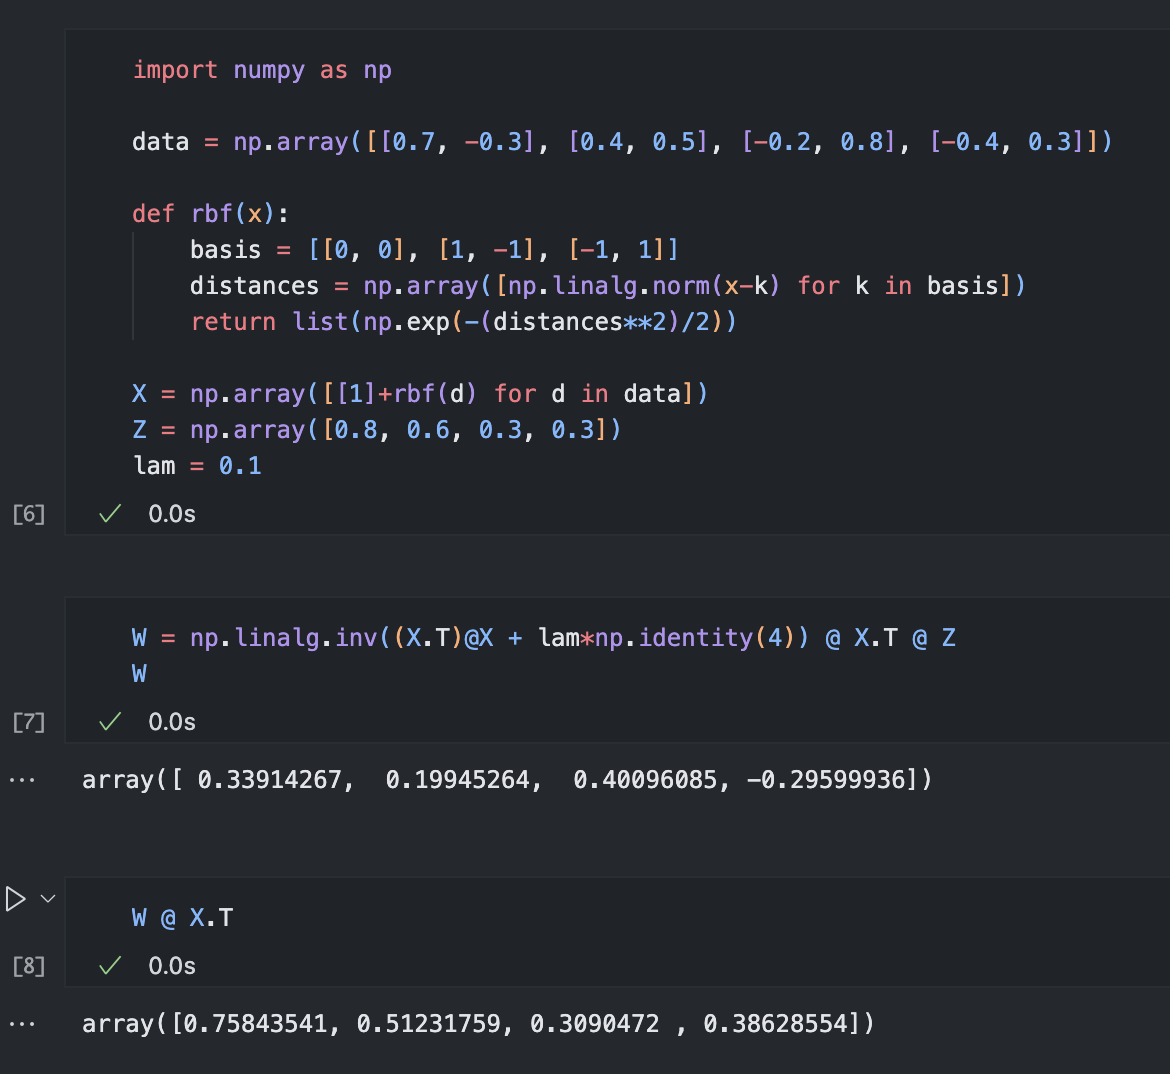
\includegraphics[scale=0.5]{images/code1.png}
        \end{center}

        Lets define the transformation of a vector as:

        \begin{equation}
            \phi(\mathbf{x}) = \begin{bmatrix}
                \phi_1(\mathbf{x}) \\
                \phi_2(\mathbf{x}) \\
                \phi_3(\mathbf{x})
            \end{bmatrix}
        \end{equation}

        Putting the new vectors into the designated matrix will give us:

        \begin{equation}
        \begin{split}
            X &= \begin{bmatrix}
                1 & \phi_1(\mathbf{x}_1) & \phi_2(\mathbf{x}_1) & \phi_3(\mathbf{x}_1) \\
                1 & \phi_1(\mathbf{x}_2) & \phi_2(\mathbf{x}_2) & \phi_3(\mathbf{x}_2) \\
                1 & \phi_1(\mathbf{x}_3) & \phi_2(\mathbf{x}_3) & \phi_3(\mathbf{x}_3) \\
                1 & \phi_1(\mathbf{x}_4) & \phi_2(\mathbf{x}_4) & \phi_3(\mathbf{x}_4)
            \end{bmatrix} \\
            &\approx \begin{bmatrix}
                1 & 0.7483 & 0.7483 & 0.1013 \\
                1 & 0.8146 & 0.2712 & 0.3312 \\
                1 & 0.7118 & 0.0963 & 0.7118 \\
                1 & 0.8825 & 0.1612 & 0.6538
            \end{bmatrix}
        \end{split}
        \end{equation}

        Since we are only transforming the input variables, our outcome values will be the same:

        \begin{equation}
            \mathbf{z} = \begin{bmatrix}
                0.8 \\
                0.6 \\
                0.3 \\
                0.3
            \end{bmatrix}
        \end{equation}

        To apply a linear regression with Ridge regularization, we want to minimize the cost function:

        \begin{equation}
            E(\mathbf{w}) = \frac{1}{2}\sum_{i=1}^{n}(z_i - \mathbf{w}^T \cdot \mathbf{x}_i)^2 + \frac{\lambda}{2} ||\mathbf{w}||^2
        \end{equation}

        The solution of this problem is the vector of weights, which is given by:

        \begin{equation}
            \mathbf{w} = \Bigl(  X^T \cdot X + \lambda I\Bigr)^{-1} \cdot X^T \cdot \mathbf{z}
        \end{equation}

        For $\lambda = 0.1$, with our data we get:

        \begin{equation}
            \mathbf{w} = \begin{bmatrix}
                0.339 & 0.199 & 0.401 & -0.296
            \end{bmatrix}
        \end{equation}

        So, our solution will be:

        \begin{equation}
        \begin{split}
            \hat{z} = f(\mathbf{x}) &= \mathbf{w} \cdot
            \begin{bmatrix}
                1 \\
                \phi_1(\mathbf{x}) \\
                \phi_2(\mathbf{x}) \\
                \phi_3(\mathbf{x})
            \end{bmatrix} \\
            &= \begin{bmatrix}
                0.339 & 0.199 & 0.401 & -0.296
            \end{bmatrix} \cdot \begin{bmatrix}
                1 \\
                \phi_1(\mathbf{x}) \\
                \phi_2(\mathbf{x}) \\
                \phi_3(\mathbf{x})
            \end{bmatrix} \\
            &= 0.339 + 0.199\phi_1(\mathbf{x}) + 0.401\phi_2(\mathbf{x}) - 0.296\phi_3(\mathbf{x})
        \end{split}
        \end{equation}

        \item Compute the training RMSE for the learnt regression.
        
        \begin{equation}
        \begin{split}
            \textrm{RMSE} &= \sqrt{\frac{1}{N}\sum_{i=1}^{N}(z_i-\hat{z}_i)^2} \\
            &= \sqrt{\frac{1}{4}\biggl( (0.8-0.7705)^2 + (0.6-0.5123)^2 + (0.3-0.3390)^2 + (0.3-0.3863)^2\biggr)} \\
            &\approx 0.06342
        \end{split}
        \end{equation}
    \end{enumerate}

    \item Consider a MLP classifier of three outcomes - $A$, $B$ and $C$ - characterized by the weights,
    \begin{equation}
        W^{[1]}=\begin{pmatrix}
            1 & 1 & 1 & 1 \\
            1 & 1 & 2 & 1 \\
            1 & 1 & 1 & 1
        \end{pmatrix}, b^{[1]} = \begin{pmatrix}
            1 \\
            1 \\
            1
        \end{pmatrix}, W^{[2]} = \begin{pmatrix}
            1 & 4 & 1 \\
            1 & 1 & 1
        \end{pmatrix}, b^{[2]} = \begin{pmatrix}
            1 \\
            1
        \end{pmatrix}, W^{[3]} = \begin{pmatrix}
            1 & 1 \\
            3 & 1 \\
            1 & 1
        \end{pmatrix}, b^{[3]} = \begin{pmatrix}
            1 \\
            1 \\
            1
        \end{pmatrix}
    \end{equation}

    the activation $f(x) = \frac{e^{0.5x-2}-e^{-0.5x+2}}{e^{0.5x-2}+e^{-0.5x+2}} = \tanh(0.5x-2)$ for every unit, and squared error loss $\frac{1}{2}||\mathbf{z}-\hat{\mathbf{z}}||^2_2$. Perform one batch gradient descent update (with learning rate $\eta = 0.1$) for training observations $\mathbf{x}_1 = (1, 1, 1, 1)$ and $\mathbf{x}_2 = (1, 0, 0, -1)$ with targets $B$ and $A$, respectively.
    
    \paragraph{Derivative of activation and loss functions:}
    \begin{equation}
    \begin{split}
        f(x) &= \tanh(0.5x-2) = \frac{e^{0.5x-2}-e^{-0.5x+2}}{e^{0.5x-2}+e^{-0.5x+2}} \\
        f'(x) &= \Biggl(\frac{e^{0.5x-2}-e^{-0.5x+2}}{e^{0.5x-2}+e^{-0.5x+2}} \Biggr)' \\
        &= \frac{\Bigl(e^{0.5x-2}-e^{-0.5x+2}\Bigr)'\Bigl(e^{0.5x-2}+e^{-0.5x+2}\Bigr)-\Bigl(e^{0.5x-2}+e^{-0.5x+2}\Bigr)'\Bigl(e^{0.5x-2}-e^{-0.5x+2}\Bigr)}{\Bigl(e^{0.5x-2}+e^{-0.5x+2}\Bigr)^2} \\
        &= \frac{\Bigl(0.5e^{0.5x-2}+0.5e^{-0.5x+2}\Bigr)\Bigl(e^{0.5x-2}+e^{-0.5x+2}\Bigr)-\Bigl(0.5e^{0.5x-2}-0.5e^{-0.5x+2}\Bigr)\Bigl(e^{0.5x-2}-e^{-0.5x+2}\Bigr)}{\Bigl(e^{0.5x-2}+e^{-0.5x+2}\Bigr)^2} \\
        &= \frac{0.5\Bigl(e^{0.5x-2}+e^{-0.5x+2}\Bigr)\Bigl(e^{0.5x-2}+e^{-0.5x+2}\Bigr)-0.5\Bigl(e^{0.5x-2}-e^{-0.5x+2}\Bigr)\Bigl(e^{0.5x-2}-e^{-0.5x+2}\Bigr)}{\Bigl(e^{0.5x-2}+e^{-0.5x+2}\Bigr)^2} \\
        &= \frac{0.5\Bigl(e^{0.5x-2}+e^{-0.5x+2}\Bigr)^2-0.5\Bigl(e^{0.5x-2}-e^{-0.5x+2}\Bigr)^2}{\Bigl(e^{0.5x-2}+e^{-0.5x+2}\Bigr)^2} \\
        &= 0.5\frac{\Bigl(e^{0.5x-2}+e^{-0.5x+2}\Bigr)^2}{\Bigl(e^{0.5x-2}+e^{-0.5x+2}\Bigr)^2} - 0.5\frac{\Bigl(e^{0.5x-2}-e^{-0.5x+2}\Bigr)^2}{\Bigl(e^{0.5x-2}+e^{-0.5x+2}\Bigr)^2}\\
        &= 0.5 - 0.5\Biggl(\frac{e^{0.5x-2}-e^{-0.5x+2}}{e^{0.5x-2}+e^{-0.5x+2}}\Biggr)^2 = 0.5 - 0.5\tanh^2(0.5x-2)
    \end{split}
    \end{equation}

    \begin{equation}
    \begin{split}
        E(\mathbf{t}, \mathbf{o}) &= \frac{1}{2}\sum_{i=1}^{k}||\mathbf{t}_i-\mathbf{o}_i||^2 \\
        \frac{\partial E}{\partial \mathbf{o}}(\mathbf{t}, \mathbf{o}) &= \frac{\partial}{\partial \mathbf{o}}\Bigl[\frac{1}{2}\sum_{i=1}^{k}||\mathbf{t}_i-\mathbf{o}_i||^2 \Bigr] \\
        &= \frac{1}{2}\sum_{i=1}^{k}\frac{\partial}{\partial \mathbf{o}_i}\Bigl[||\mathbf{t}_i-\mathbf{o}_i||^2 \Bigr] \\
        &= \frac{1}{2}\sum_{i=1}^{k}\Bigl[ 2(\mathbf{t}_i - \mathbf{o}_i)\cdot(-1)\Bigr] \\
        &= -\sum_{i=1}^{k}(\mathbf{t}_i - \mathbf{o}_i)
    \end{split}
    \end{equation}

    For this neural network, since the output layer has index 3, then $\mathbf{o} = \mathbf{x}^{[3]}$.

    \begin{center}
        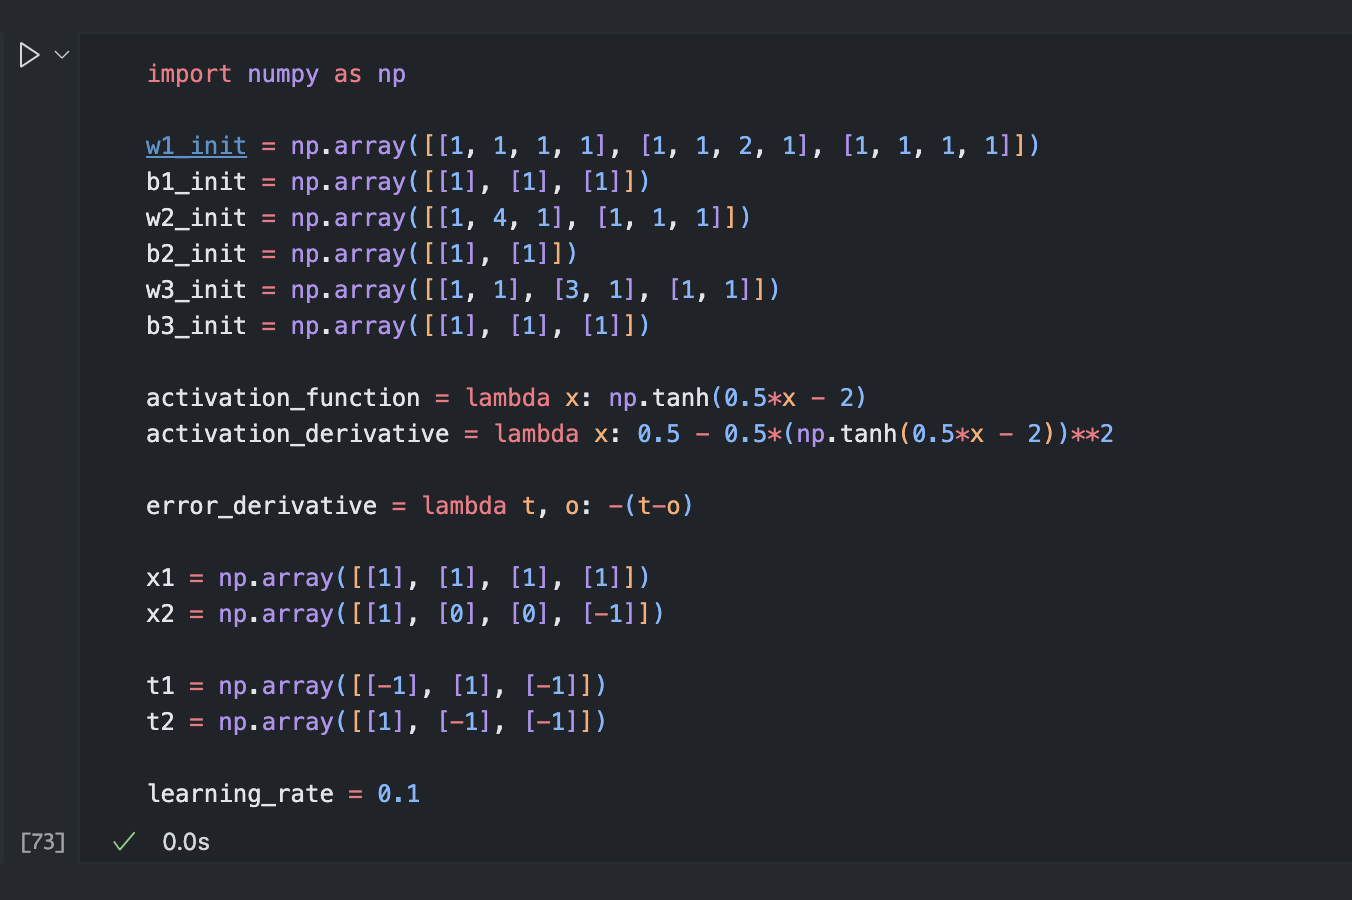
\includegraphics[scale=0.5]{images/code2.png}
    \end{center}

    \paragraph{Notation:} Since the derivative of the sum is the sum of the derivatives, we will compute the contribuitions for the gradient descent individually for each observation. That way, lets define $\mathbf{y}_i^{[j]}$ as the contribuition of the $i$th observation to $\mathbf{y}$ component (can be a vector or matrix) of the $j$th layer. While $\mathbf{y}^{[j]}$ means the overall contribuition to the $\mathbf{y}$ component of the $j$th layer.

    \paragraph{Forward propagation:} Firstly we will need to forward propagate in order to get the prediction for the observations using the old weights and biases.
    The base rules for forward propagation are:

    \begin{equation}
    \begin{split}
        \mathbf{z}^{[k]} &= \mathbf{W}^{[k]} \cdot \mathbf{x}^{[k-1]} + \mathbf{b}^{[k]} \\
        \mathbf{x}^{[k]} &= \phi^{[k]}(\mathbf{z}^{[k]})
    \end{split}
    \end{equation}

    Where $\mathbf{x}^{[0]} = \mathbf{x}$, $\hat{\mathbf{z}} = \mathbf{x}^{[k]}$ (where $k$ is the last layer's index). $\phi^{[k]}$ is the activation function for the $k$th layer applied element wise, in this case $\phi^{[k]}(x) = f(x) =\tanh(0.5x-2)$ for every $k$.

    \begin{center}
        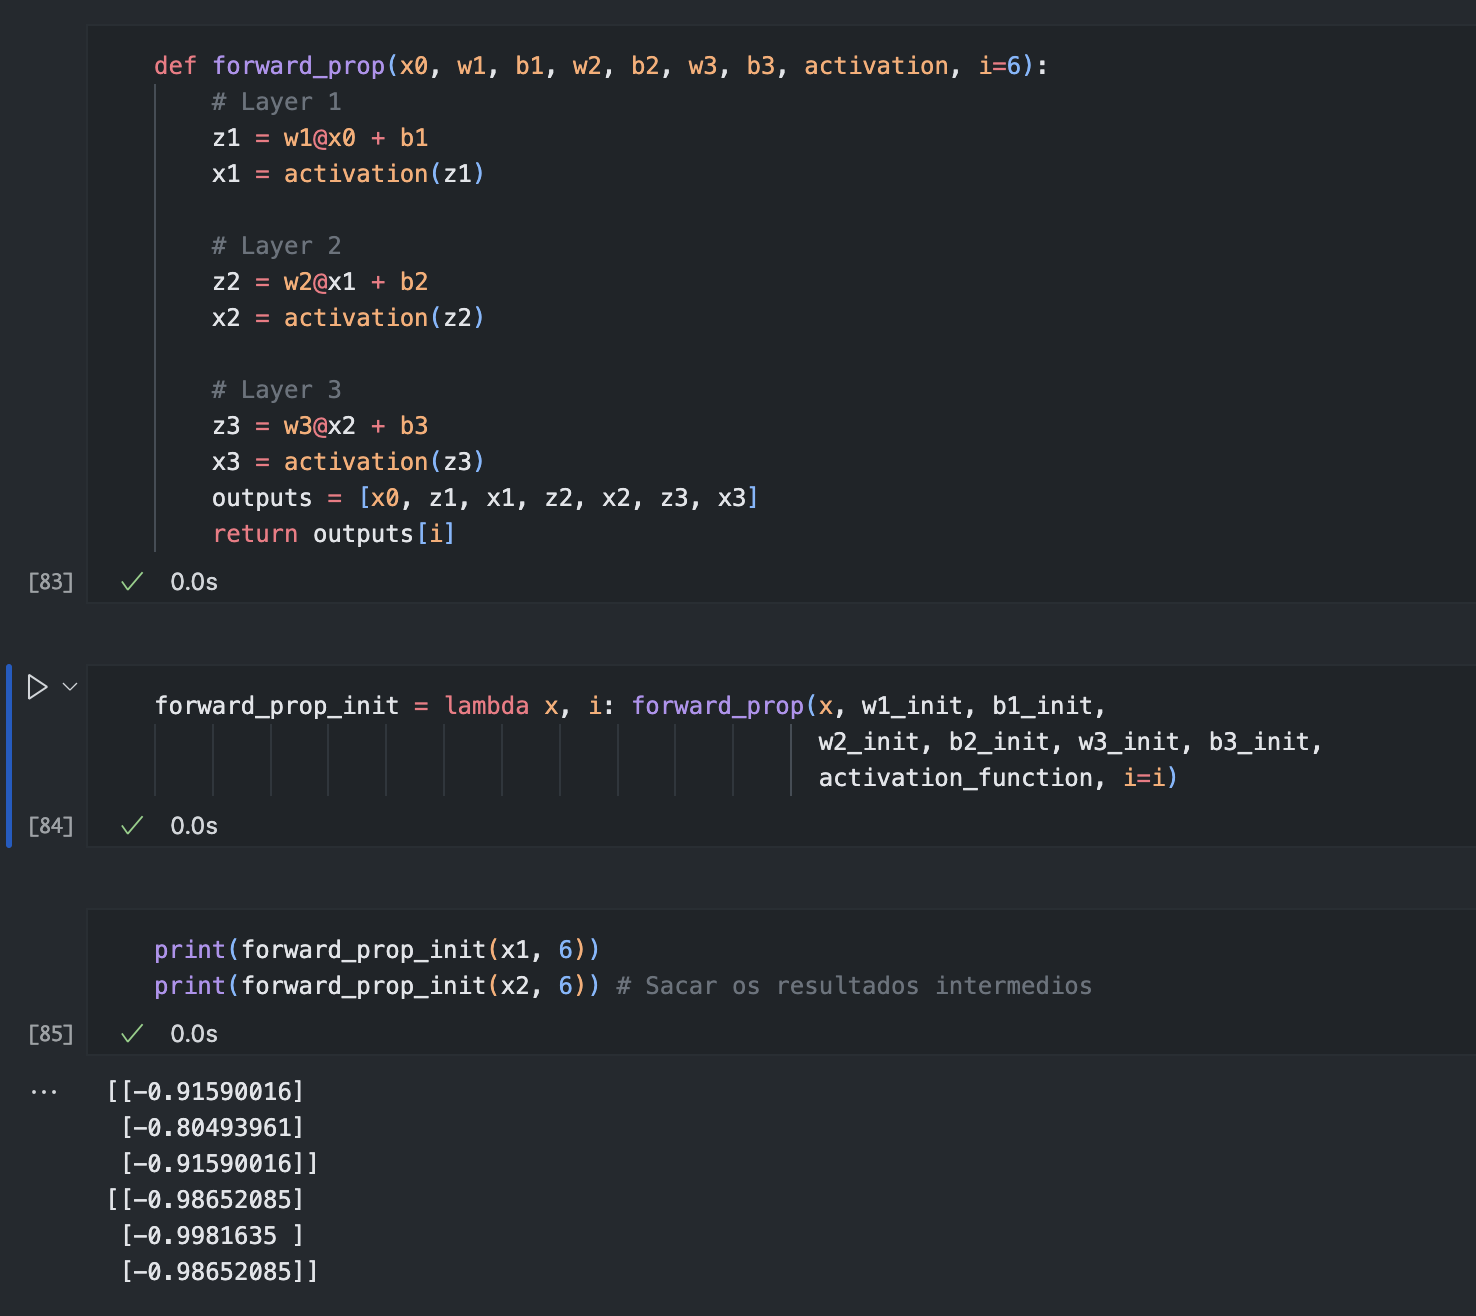
\includegraphics[scale=0.4]{images/code3.png}
    \end{center}

    \begin{equation}
    \begin{aligned}
        \mathbf{x}_1^{[0]} &= \begin{bmatrix}
            1 \\ 1 \\ 1 \\ 1
        \end{bmatrix} &\qquad \mathbf{x}_2^{[0]} &= \begin{bmatrix}
            1 \\ 0 \\ 0 \\ -1
        \end{bmatrix} \\
        \mathbf{z}_1^{[1]} &= \mathbf{W}^{[1]} \cdot \mathbf{x}_1^{[0]} + \mathbf{b}^{[1]} = \begin{bmatrix}
            5 \\ 6 \\ 5
        \end{bmatrix} &\qquad \mathbf{z}_2^{[1]} &= \mathbf{W}^{[1]} \cdot \mathbf{x}_2^{[0]} + \mathbf{b}^{[1]} = \begin{bmatrix}
            1 \\ 1 \\ 1
        \end{bmatrix} \\
        \mathbf{x}_1^{[1]} &= \phi^{[1]}(\mathbf{z}_1^{[1]}) = f(\mathbf{z}_1^{[1]}) \approx \begin{bmatrix}
            0.4621 \\ 0.7616 \\ 0.4621
        \end{bmatrix}&\qquad \mathbf{x}_2^{[1]} &= \phi^{[1]}(\mathbf{z}_2^{[1]}) = f(\mathbf{z}_2^{[1]}) \approx \begin{bmatrix}
            -0.9051 \\ -0.9051 \\ -0.9051
        \end{bmatrix} \\
        \mathbf{z}_1^{[2]} &= \mathbf{W}^{[2]} \cdot \mathbf{x}_1^{[1]} + \mathbf{b}^{[2]} \approx \begin{bmatrix}
            4.9706 \\ 2.6858
        \end{bmatrix} &\qquad \mathbf{z}_2^{[2]} &= \mathbf{W}^{[2]} \cdot \mathbf{x}_2^{[1]} + \mathbf{b}^{[2]} \approx \begin{bmatrix}
            -4.4309 \\ -1.7154
        \end{bmatrix} \\
        \mathbf{x}_1^{[2]} &= \phi^{[2]}(\mathbf{z}_1^{[2]}) = f(\mathbf{z}_1^{[2]}) \approx \begin{bmatrix}
            0.4505 \\ -0.5764
        \end{bmatrix}&\qquad \mathbf{x}_2^{[2]} &= \phi^{[2]}(\mathbf{z}_2^{[2]}) = f(\mathbf{z}_2^{[2]}) \approx \begin{bmatrix}
            -0.9996 \\ -0.9934
        \end{bmatrix} \\
        \mathbf{z}_1^{[3]} &= \mathbf{W}^{[3]} \cdot \mathbf{x}_1^{[2]} + \mathbf{b}^{[3]} \approx \begin{bmatrix}
            0.8741 \\ 1.7750 \\ 0.8741
        \end{bmatrix} &\qquad \mathbf{z}_2^{[3]} &= \mathbf{W}^{[3]} \cdot \mathbf{x}_2^{[2]} + \mathbf{b}^{[3]} \approx \begin{bmatrix}
            -0.9930 \\ -2.9921 \\ -0.9930
        \end{bmatrix} \\
        \mathbf{x}_1^{[3]} &= \phi^{[3]}(\mathbf{z}_1^{[3]}) = f(\mathbf{z}_1^{[3]}) \approx \begin{bmatrix}
            -0.9159 \\ -0.8049 \\ -0.9159
        \end{bmatrix} &\qquad \mathbf{x}_2^{[3]} &= \phi^{[3]}(\mathbf{z}_2^{[3]}) = f(\mathbf{z}_2^{[3]}) \approx \begin{bmatrix}
            -0.9865 \\ -0.9982 \\ -0.9865
        \end{bmatrix}
    \end{aligned}
    \end{equation}

    \paragraph{Class encoding} Since Neural Networks operate solely on numbers, we need to define an encoding for the output. The way to encode the classes is to have the number of output layer neurons equal to the number of classes, and for the $k$th class the encoding have the max value possible on the $k$th coordinate and the minimum value possible on the other coordinates. Since the activation function of the output layer is $\tanh(x) \in [-1, 1]$, we have:

    \begin{equation}
    \begin{aligned}
        \hat{z} = A \Rightarrow t = \begin{bmatrix}
            1 \\ -1 \\ -1
        \end{bmatrix} &\qquad \hat{z} = B \Rightarrow t = \begin{bmatrix}
            -1 \\ 1 \\ -1
        \end{bmatrix} &\qquad \hat{z} = C \Rightarrow t = \begin{bmatrix}
            -1 \\ -1 \\ 1
        \end{bmatrix}
    \end{aligned}
    \end{equation}

    That way, for our observations, we have:

    \begin{equation}
    \begin{aligned}
        \hat{z}_1 = B \Rightarrow t_1 = \begin{bmatrix}
            -1 \\ 1 \\ -1
        \end{bmatrix} \qquad\qquad\qquad \hat{z}_2 = A \Rightarrow t_2 = \begin{bmatrix}
            1 \\ -1 \\ -1
        \end{bmatrix}
    \end{aligned}
    \end{equation}

    \paragraph{Backpropagation rules:} The base of Backpropagation is the following rule:

    \begin{equation}
        \mathbf{W}^{[k]} = \mathbf{W}^{[k]} - \eta\frac{\partial E}{\partial \mathbf{W}^{[k]}}
    \end{equation}

    The same applies for the biases:

    \begin{equation}
        \mathbf{b}^{[k]} = \mathbf{b}^{[k]} - \eta\frac{\partial E}{\partial \mathbf{b}^{[k]}}
    \end{equation}

    If the $k$th layer is the last, we have:

    \begin{equation}
    \begin{aligned}
        \frac{\partial E}{\partial \mathbf{W}^{[k]}} &= \frac{\partial E}{\partial \mathbf{x}^{[k]}} \circ \frac{\partial \mathbf{x}^{[k]}}{\partial \mathbf{z}^{[k]}} \cdot \frac{\partial \mathbf{z}^{[k]}}{\partial \mathbf{W}^{[k]}} \\
        &= \frac{\partial E}{\partial \mathbf{x}^{[k]}} \circ \phi'^{[k]}(\mathbf{z}^{[k]}) \cdot \mathbf{x}^{[k-1]}
    \end{aligned}
    \end{equation}

    \begin{equation}
    \begin{aligned}
        \frac{\partial E}{\partial \mathbf{b}^{[k]}} &= \frac{\partial E}{\partial \mathbf{x}^{[k]}} \circ \frac{\partial \mathbf{x}^{[k]}}{\partial \mathbf{z}^{[k]}} \cdot \frac{\partial \mathbf{z}^{[k]}}{\partial \mathbf{b}^{[k]}} \\
        &= \frac{\partial E}{\partial \mathbf{x}^{[k]}} \circ \phi'^{[k]}(\mathbf{z}^{[k]})
    \end{aligned}
    \end{equation}

    By defining, for any layer of index $i$ on a network with $k+1$ layers (last layer has index $k$):

    \begin{equation}
        \delta^{[i]} = \left\{
        \begin{array}{ll}
            \frac{\partial E}{\partial \mathbf{x}^{[k]}} \circ \phi'^{[k]}(\mathbf{z}^{[k]}) & \textrm{if} \quad i = k \\
            \\
            {\mathbf{W}^{[i+1]}}^T \cdot \delta^{[i+1]} \circ \phi'^{[i]}(\mathbf{z}^{[i]})  & \textrm{else}
        \end{array} 
        \right.
    \end{equation}

    We can write:

    \begin{equation}
    \begin{aligned}
        \frac{\partial E}{\partial \mathbf{W}^{[i]}} &= \delta^{[i]} \cdot {(\mathbf{x}^{[i-1]})}^T \\
        \frac{\partial E}{\partial \mathbf{b}^{[i]}} &= \delta^{[i]} \\
    \end{aligned}
    \end{equation}

    \paragraph{Backpropagation:}

    \begin{center}
        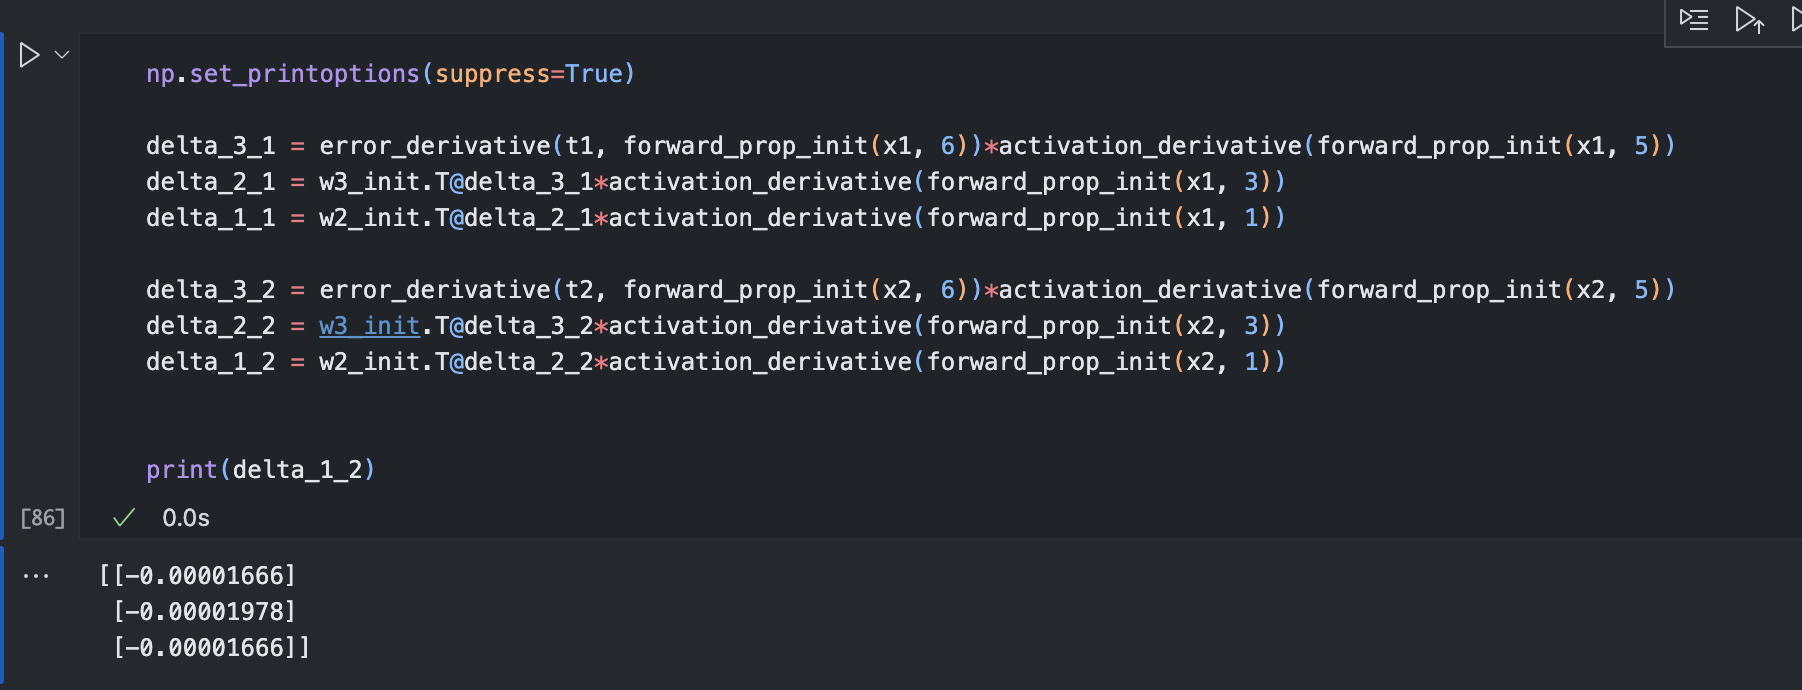
\includegraphics[scale=0.4]{images/code4.png}
    \end{center}

    \begin{equation}
    \begin{aligned}
        \delta_1^{[3]} &= \frac{\partial E}{\partial \mathbf{x}_1^{[3]}} \circ \phi'^{[3]}(\mathbf{z}_1^{[3]}) = -(\mathbf{t}_1 - \mathbf{x}_1^{[3]}) \circ \begin{bmatrix}            f'(0.8741) \\ f'(1.7750) \\ f'(0.8741)
        \end{bmatrix} = \begin{bmatrix}
            0.00677537 \\ -0.31773455 \\ 0.00677537
        \end{bmatrix} \\
        \delta_2^{[3]} &= \frac{\partial E}{\partial \mathbf{x}_2^{[3]}} \circ \phi'^{[3]}(\mathbf{z}_2^{[3]}) = \begin{bmatrix}
            -0.02659614 \\ 0.00000337 \\ 0.00018046
        \end{bmatrix}
    \end{aligned}
    \end{equation}

    \begin{equation}
    \begin{aligned}
        \delta_1^{[2]} &= {\mathbf{W}^{[3]}}^T \cdot \delta_1^{[3]} \circ \phi'^{[2]}(\mathbf{z}_1^{[2]})
        &= \begin{bmatrix}
            -0.37448246 \\ -0.10155772
        \end{bmatrix} \\
        \delta_2^{[2]} &= {\mathbf{W}^{[3]}}^T \cdot \delta_2^{[3]} \circ \phi'^{[2]}(\mathbf{z}_2^{[2]})
        &= \begin{bmatrix}
            -0.00001151 \\ -0.0001729 
        \end{bmatrix} \\
        \delta_1^{[1]} &= {\mathbf{W}^{[2]}}^T \cdot \delta_1^{[2]} \circ \phi'^{[1]}(\mathbf{z}_1^{[1]})
        &= \begin{bmatrix}
            -0.18719036 \\ -0.33587187 \\ -0.18719036
        \end{bmatrix} \\
        \delta_2^{[1]} &= {\mathbf{W}^{[2]}}^T \cdot \delta_2^{[2]} \circ \phi'^{[1]}(\mathbf{z}_2^{[1]})
        &= \begin{bmatrix}
            -0.00001666 \\ -0.00001978 \\ -0.00001666
        \end{bmatrix}
    \end{aligned}
    \end{equation}

    \begin{center}
        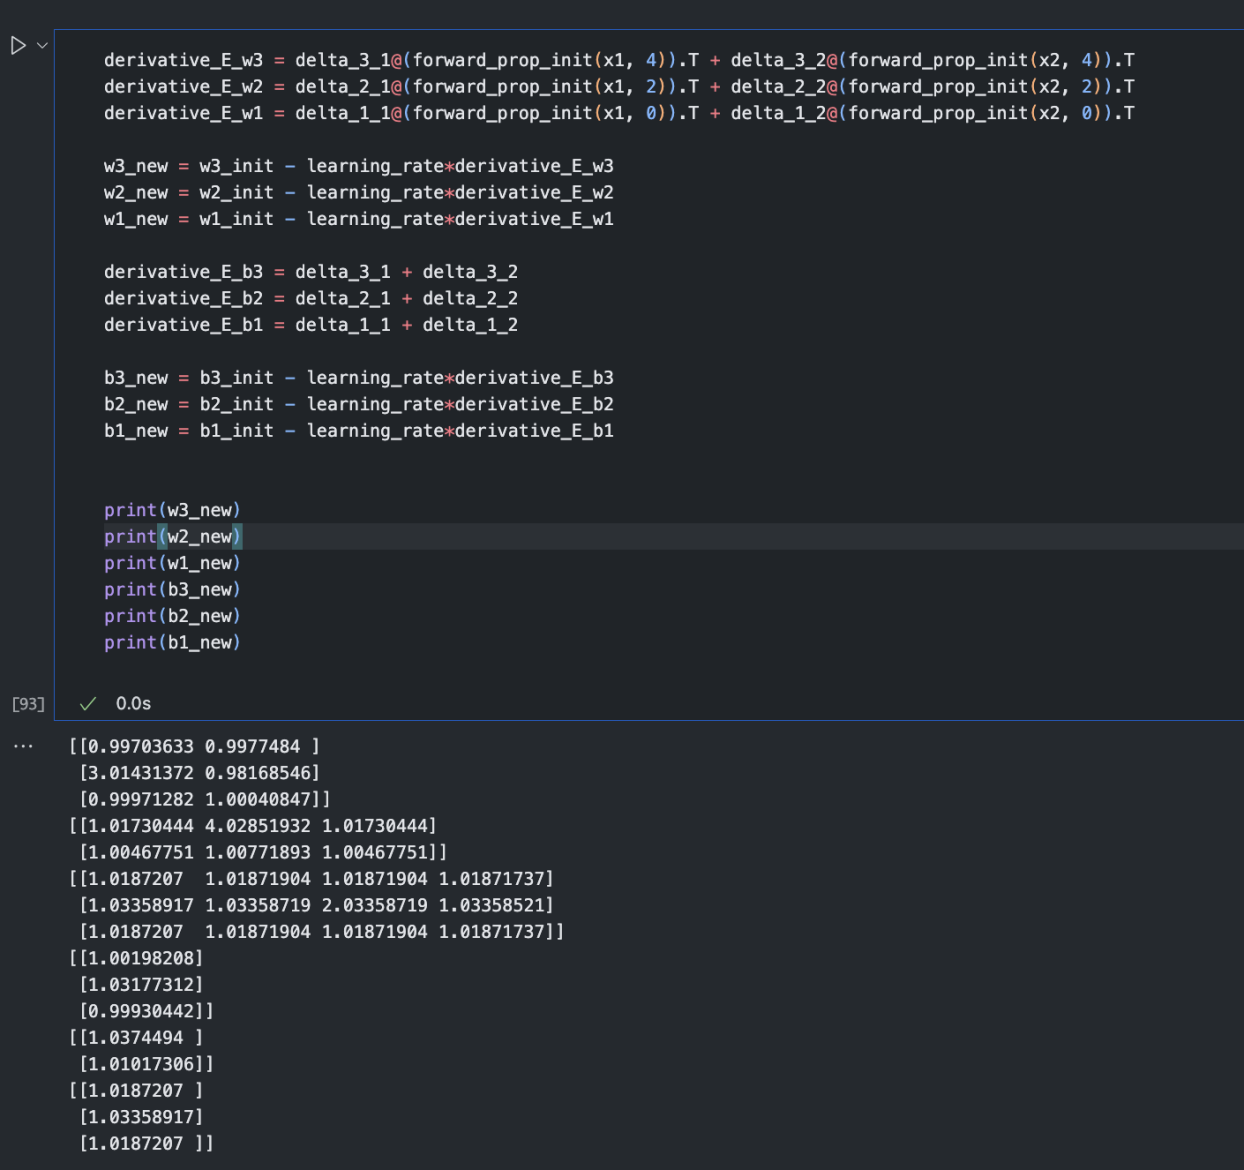
\includegraphics[scale=0.3]{images/code5.png}
    \end{center}

    \begin{equation}
    \begin{aligned}
        \frac{\partial E}{\partial \mathbf{W}^{[3]}} &= \delta^{[3]} \cdot (\mathbf{x}^{[2]})^T = \delta_1^{[3]} \cdot (\mathbf{x}_1^{[2]})^T + \delta_2^{[3]} \cdot (\mathbf{x}_2^{[2]})^T \\
        &= \begin{bmatrix}
            0.02963673 & 0.022516 \\
            -0.14313723 & 0.18314544 \\
             0.0028718 & -0.00408474
        \end{bmatrix} \\
        \frac{\partial E}{\partial \mathbf{W}^{[2]}} &= \delta^{[2]} \cdot (\mathbf{x}^{[1]})^T = \delta_1^{[2]} \cdot (\mathbf{x}_1^{[1]})^T + \delta_2^{[2]} \cdot (\mathbf{x}_2^{[1]})^T \\
        &= \begin{bmatrix}
            -0.17304435 & -0.28519324 & -0.17304435 \\
            -0.04677506 & -0.07718926 & -0.04677506
        \end{bmatrix} \\
        \frac{\partial E}{\partial \mathbf{W}^{[1]}} &= \delta^{[1]} \cdot (\mathbf{x}^{[0]})^T = \delta_1^{[1]} \cdot (\mathbf{x}_1^{[0]})^T + \delta_2^{[1]} \cdot (\mathbf{x}_2^{[0]})^T \\
        &= \begin{bmatrix}
            -0.18720702 & -0.18719036 & -0.18719036 & -0.1871737 \\
            -0.33589165 & -0.33587187 & -0.33587187 & -0.33585209 \\
            -0.18720702 & -0.18719036 & -0.18719036 & -0.1871737 \\
        \end{bmatrix}
    \end{aligned}
    \end{equation}

    \begin{equation}
    \begin{aligned}
        \frac{\partial E}{\partial \mathbf{b}^{[3]}} &= \delta^{[3]} = \delta_1^{[3]} + \delta_2^{[3]} \\
        &= \begin{bmatrix}
            -0.01982077 \\-0.31773118 \\ 0.00695584
        \end{bmatrix} \\
        \frac{\partial E}{\partial \mathbf{b}^{[2]}} &= \delta^{[2]} = \delta_1^{[2]} + \delta_2^{[2]} \\
        &= \begin{bmatrix}
            -0.37449397 \\ -0.10173062
        \end{bmatrix} \\
        \frac{\partial E}{\partial \mathbf{b}^{[1]}} &= \delta^{[1]} = \delta_1^{[1]} + \delta_2^{[1]} \\
        &= \begin{bmatrix}
            -0.18720702 \\ -0.33589165 \\ -0.18720702
        \end{bmatrix} \\
    \end{aligned}
    \end{equation}

    \begin{equation}
    \begin{aligned}
        \mathbf{W}_{new}^{[3]} &= \mathbf{W}^{[3]} - \eta \frac{\partial E}{\partial \mathbf{W}^{[3]}}
        = \begin{bmatrix}
            0.99703633 & 0.9977484 \\
            3.01431372 & 0.98168546 \\
            0.99971282 & 1.00040847 \\
            \end{bmatrix} \\
        \mathbf{W}_{new}^{[2]} &= \mathbf{W}^{[2]} - \eta \frac{\partial E}{\partial \mathbf{W}^{[2]}}
        = \begin{bmatrix}
            1.01730444 & 4.02851932 & 1.01730444 \\
            1.00467751 & 1.00771893 & 1.00467751
        \end{bmatrix} \\
        \mathbf{W}_{new}^{[1]} &= \mathbf{W}^{[1]} - \eta \frac{\partial E}{\partial \mathbf{W}^{[1]}}
        = \begin{bmatrix}
            1.0187207  & 1.01871904 & 1.01871904 & 1.01871737 \\
            1.03358917 & 1.03358719 & 2.03358719 & 1.03358521 \\
            1.0187207  & 1.01871904 & 1.01871904 & 1.01871737 \\
            \end{bmatrix}
    \end{aligned}
    \end{equation}

    \begin{equation}
    \begin{aligned}
        \mathbf{b}_{new}^{[3]} &= \mathbf{b}^{[3]} - \eta \frac{\partial E}{\partial \mathbf{b}^{[3]}}
        = \begin{bmatrix}
            1.00198208 \\ 1.03177312 \\ 0.99930442
            \end{bmatrix} \\
        \mathbf{b}_{new}^{[2]} &= \mathbf{b}^{[2]} - \eta \frac{\partial E}{\partial \mathbf{b}^{[2]}}
        = \begin{bmatrix}
            1.0374494 \\ 1.01017306
        \end{bmatrix} \\
        \mathbf{b}_{new}^{[1]} &= \mathbf{b}^{[1]} - \eta \frac{\partial E}{\partial \mathbf{b}^{[1]}}
        = \begin{bmatrix}
            1.0187207 \\ 1.03358917 \\ 1.0187207 
            \end{bmatrix}
    \end{aligned}
    \end{equation}

\end{enumerate}

\vskip 1cm

\large{\textbf{Part II}: Programming and Critical Analysis}\normalsize







\end{document}
